\begin{figure*}

\begin{subfigure}{0.5\textwidth}
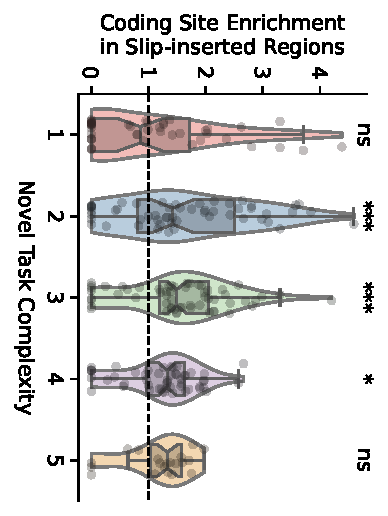
\includegraphics[height=\textwidth,angle=90]{binder/binder/teeplots/density-norm=width+hue=components+viability=exclude+viz=violinplot+x=components+y=is-task-coding-site+ext=.pdf}
\caption{%
\footnotesize
excluding sites critical to survival
}
\end{subfigure}%
% \begin{subfigure}{0.5\textwidth}
% 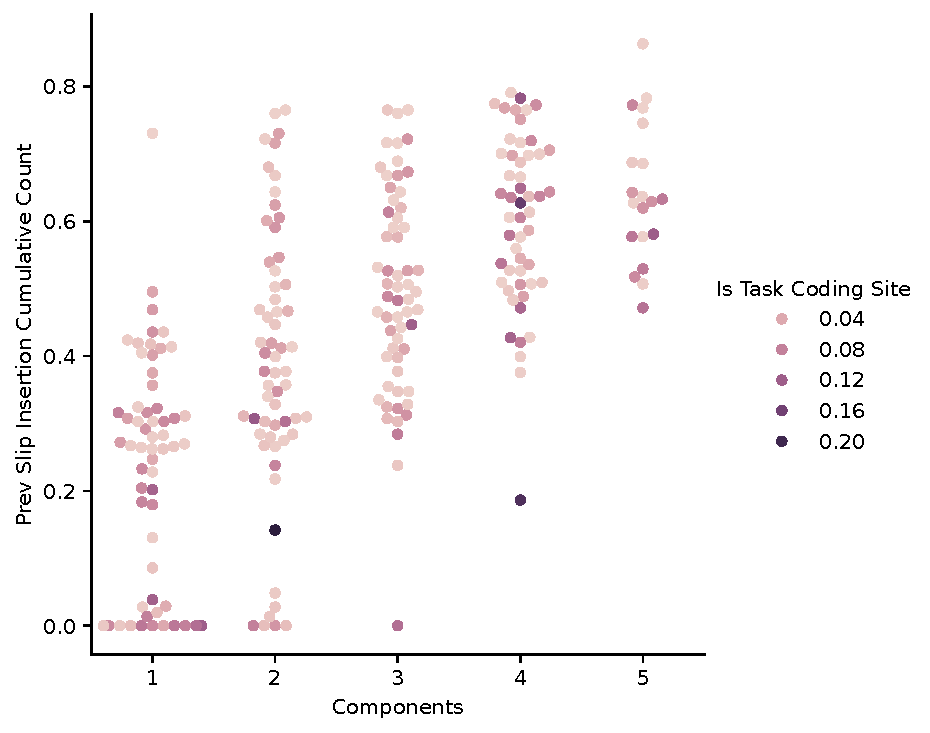
\includegraphics[width=\textwidth]{binder/binder/teeplots/hue=is-task-coding-site+kind=swarm+viz=catplot+x=components+y=prev-slip-insertion-cumulative-count+ext=.pdf}
% \caption{%
% \footnotesize
% Ratios of slip-duplicated to non-slip-duplicated sites for observed gain-of-function events.
% }
% \end{subfigure}
% \begin{subfigure}{0.5\textwidth}
% 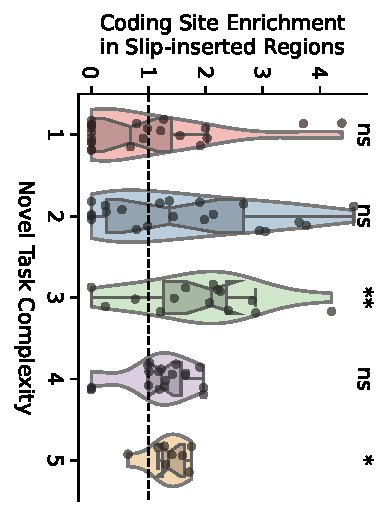
\includegraphics[height=\textwidth,angle=90]{binder/binder/teeplots/density-norm=width+hue=components+slipgain=only+viz=violinplot+x=components+y=is-task-coding-site+ext=.pdf}
% \caption{%
% \footnotesize
% for gain-of-function events immediately coincident with slip duplication events.
% }
% \end{subfigure}
\begin{subfigure}{0.5\textwidth}
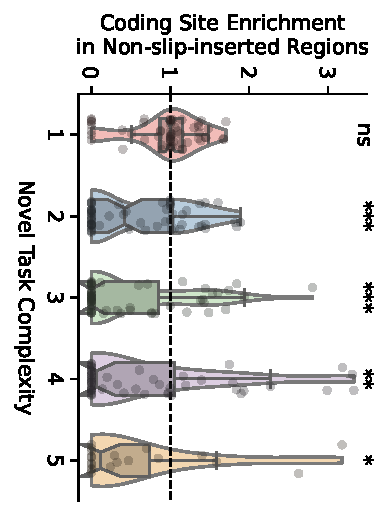
\includegraphics[height=\textwidth,angle=90]{binder/binder/teeplots/density-norm=width+hue=components+viz=violinplot+what=base-negated+x=components+y=is-task-coding-site+ext=.pdf}
\caption{%
\footnotesize
coding site enrichment in \textit{non-slip-duplicated} regions
}
\label{fig:potentiation-supp:non-slip-dup}
\end{subfigure}

\begin{subfigure}{0.5\textwidth}
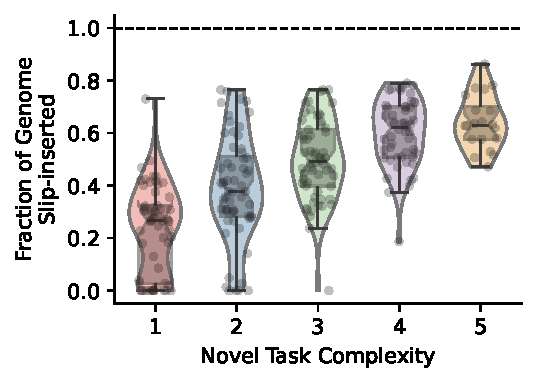
\includegraphics[width=\textwidth]{binder/binder/teeplots/density-norm=width+hue=components+viz=violinplot+what=frac-slip-duplicated+x=components+y=prev-slip-insertion-cumulative-count+ext=.pdf}
\caption{%
\footnotesize
fraction of genome that has been slip-duplicated
}
\label{fig:potentiation-supp:frac-slip-dup}
\end{subfigure}

\caption{%
\textbf{Slip-duplication potentiation analysis detail.}
Panel \ref{fig:excluding sites critical to survival} shows coding site enrichment for \textit{de novo} logic-9 tasks in slip-duplicated regions, excluding sites assessed by knockout analysis as critical to self-copy loop viability.
Plot composition follows \ref{fig:potentiation}, with values greater than 1 indicating that coding sites of novel traits occur more often in slip-duplicated regions compared to their background frequency.
  Significance of deviation from null expectation median value of 1.0 is indicated with * ($p < 0.05$), ** ($p < 0.01$), or *** ($p < 0.001$) (one-tailed Wilcoxon signed-rank test).
  Panels \cref{fig:potentiation-supp:non-slip-dup,fig:potentiation-supp:frac-slip-dup} provide additional context, showing coding site enrichment values for \textit{non-}duplicated sites and the overall fraction of the genome that has been slip-duplicated.
}
\label{fig:potentiation-supp}
\end{figure*}



% https://github.com/chaynes2019/AvidaGeneDupe/blob/4c7fa27229094adcb5bdb0b1aec541d0014b0fed/binder/hard-task-gain.ipynb
%             H-statistic       p-value
% Components
% 1              0.852615  3.558135e-01
% 2             22.275265  2.362300e-06
% 3             30.283198  3.733461e-08
% 4             15.404583  8.677756e-05
% 5              7.425000  6.432383e-03
%    Components  Prev Slip Insertion Cumulative Count      mean       std
% 0           1                                 False  1.021203  0.539732
% 1           1                                  True  1.049763  1.171343
% 2           2                                 False  0.633574  0.681144
% 3           2                                  True  1.621013  1.183828
% 4           3                                 False  0.546084  0.783429
% 5           3                                  True  1.530474  0.918999
% 6           4                                 False  0.700892  1.021518
% 7           4                                  True  1.234347  0.656445
% 8           5                                 False  0.616704  0.989464
% 9           5                                  True  1.176742  0.596213
%    Components  Prev Slip Insertion Cumulative Count  size
% 0           1                                 False    60
% 1           1                                  True    46
% 2           2                                 False    60
% 3           2                                  True    55
% 4           3                                 False    60
% 5           3                                  True    59
% 6           4                                 False    52
% 7           4                                  True    52
% 8           5                                 False    20
% 9           5                                  True    20
